% !TeX root = ../main.tex
\section{Experiments}
\label{sec:experiments}

\textcolor{red}{This section evaluates the proposed method in terms of prediction accuracy, conditional controllability, ablation behavior, computational efficiency, and engineering feasibility.}

\subsection{Experimental setup}
\label{subsec:exp_setup}

\textcolor{red}{The experimental setup first describes the dataset and condition grouping, then introduces the baseline, implementation settings, and evaluation metrics used for comparison.}

\subsubsection{Dataset}
\label{subsubsec:dataset}

\begin{table}[t]
\centering
\caption{Dataset statistics}
\label{tab:dataset_stats}
\begin{tabularx}{\columnwidth}{lX}
\toprule
Statistic & Value \\
\midrule
Total floor plans & 143 \\
Condition distribution (Low:Med:High) & 33 : 52 : 58 \\
Train / Test split & 80\% / 20\% \\
Avg. rooms per floor plan & 26.5 \\
Avg. edges per graph & 71.6 \\
Samples after augmentation (train) & 678 \\
\bottomrule
\end{tabularx}
\end{table}


\begin{table*}[t]
\centering
\begingroup\color{red}
\caption{Sensitivity of CGS to alternative component weights}
\label{tab:cgs_sensitivity}
\begin{tabular*}{\textwidth}{@{\extracolsep{\fill}}lcccc@{}}
\toprule
Weight setting & Full model & w/o FiLM & w/o dual-stream & w/o density loss \\
\midrule
Equal weights $(1/3,1/3,1/3)$ & 0.708 & 0.700 & 0.692 & 0.651 \\
Density-oriented $(0.5,0.25,0.25)$ & 0.713 & 0.713 & 0.702 & 0.640 \\
Geometry-oriented $(0.25,0.5,0.25)$ & 0.661 & 0.652 & 0.650 & 0.624 \\
Uniformity-oriented $(0.25,0.25,0.5)$ & 0.729 & 0.715 & 0.725 & 0.690 \\
\bottomrule
\end{tabular*}
\endgroup
\end{table*}


\begin{figure*}[t]
\centering

\includegraphics[width=0.9\textwidth]{qual_comparison.png}
\caption{Comparison of qualitative prediction results.}
\label{fig:qual_comparison}
\end{figure*}

\begin{figure*}[t]
\centering
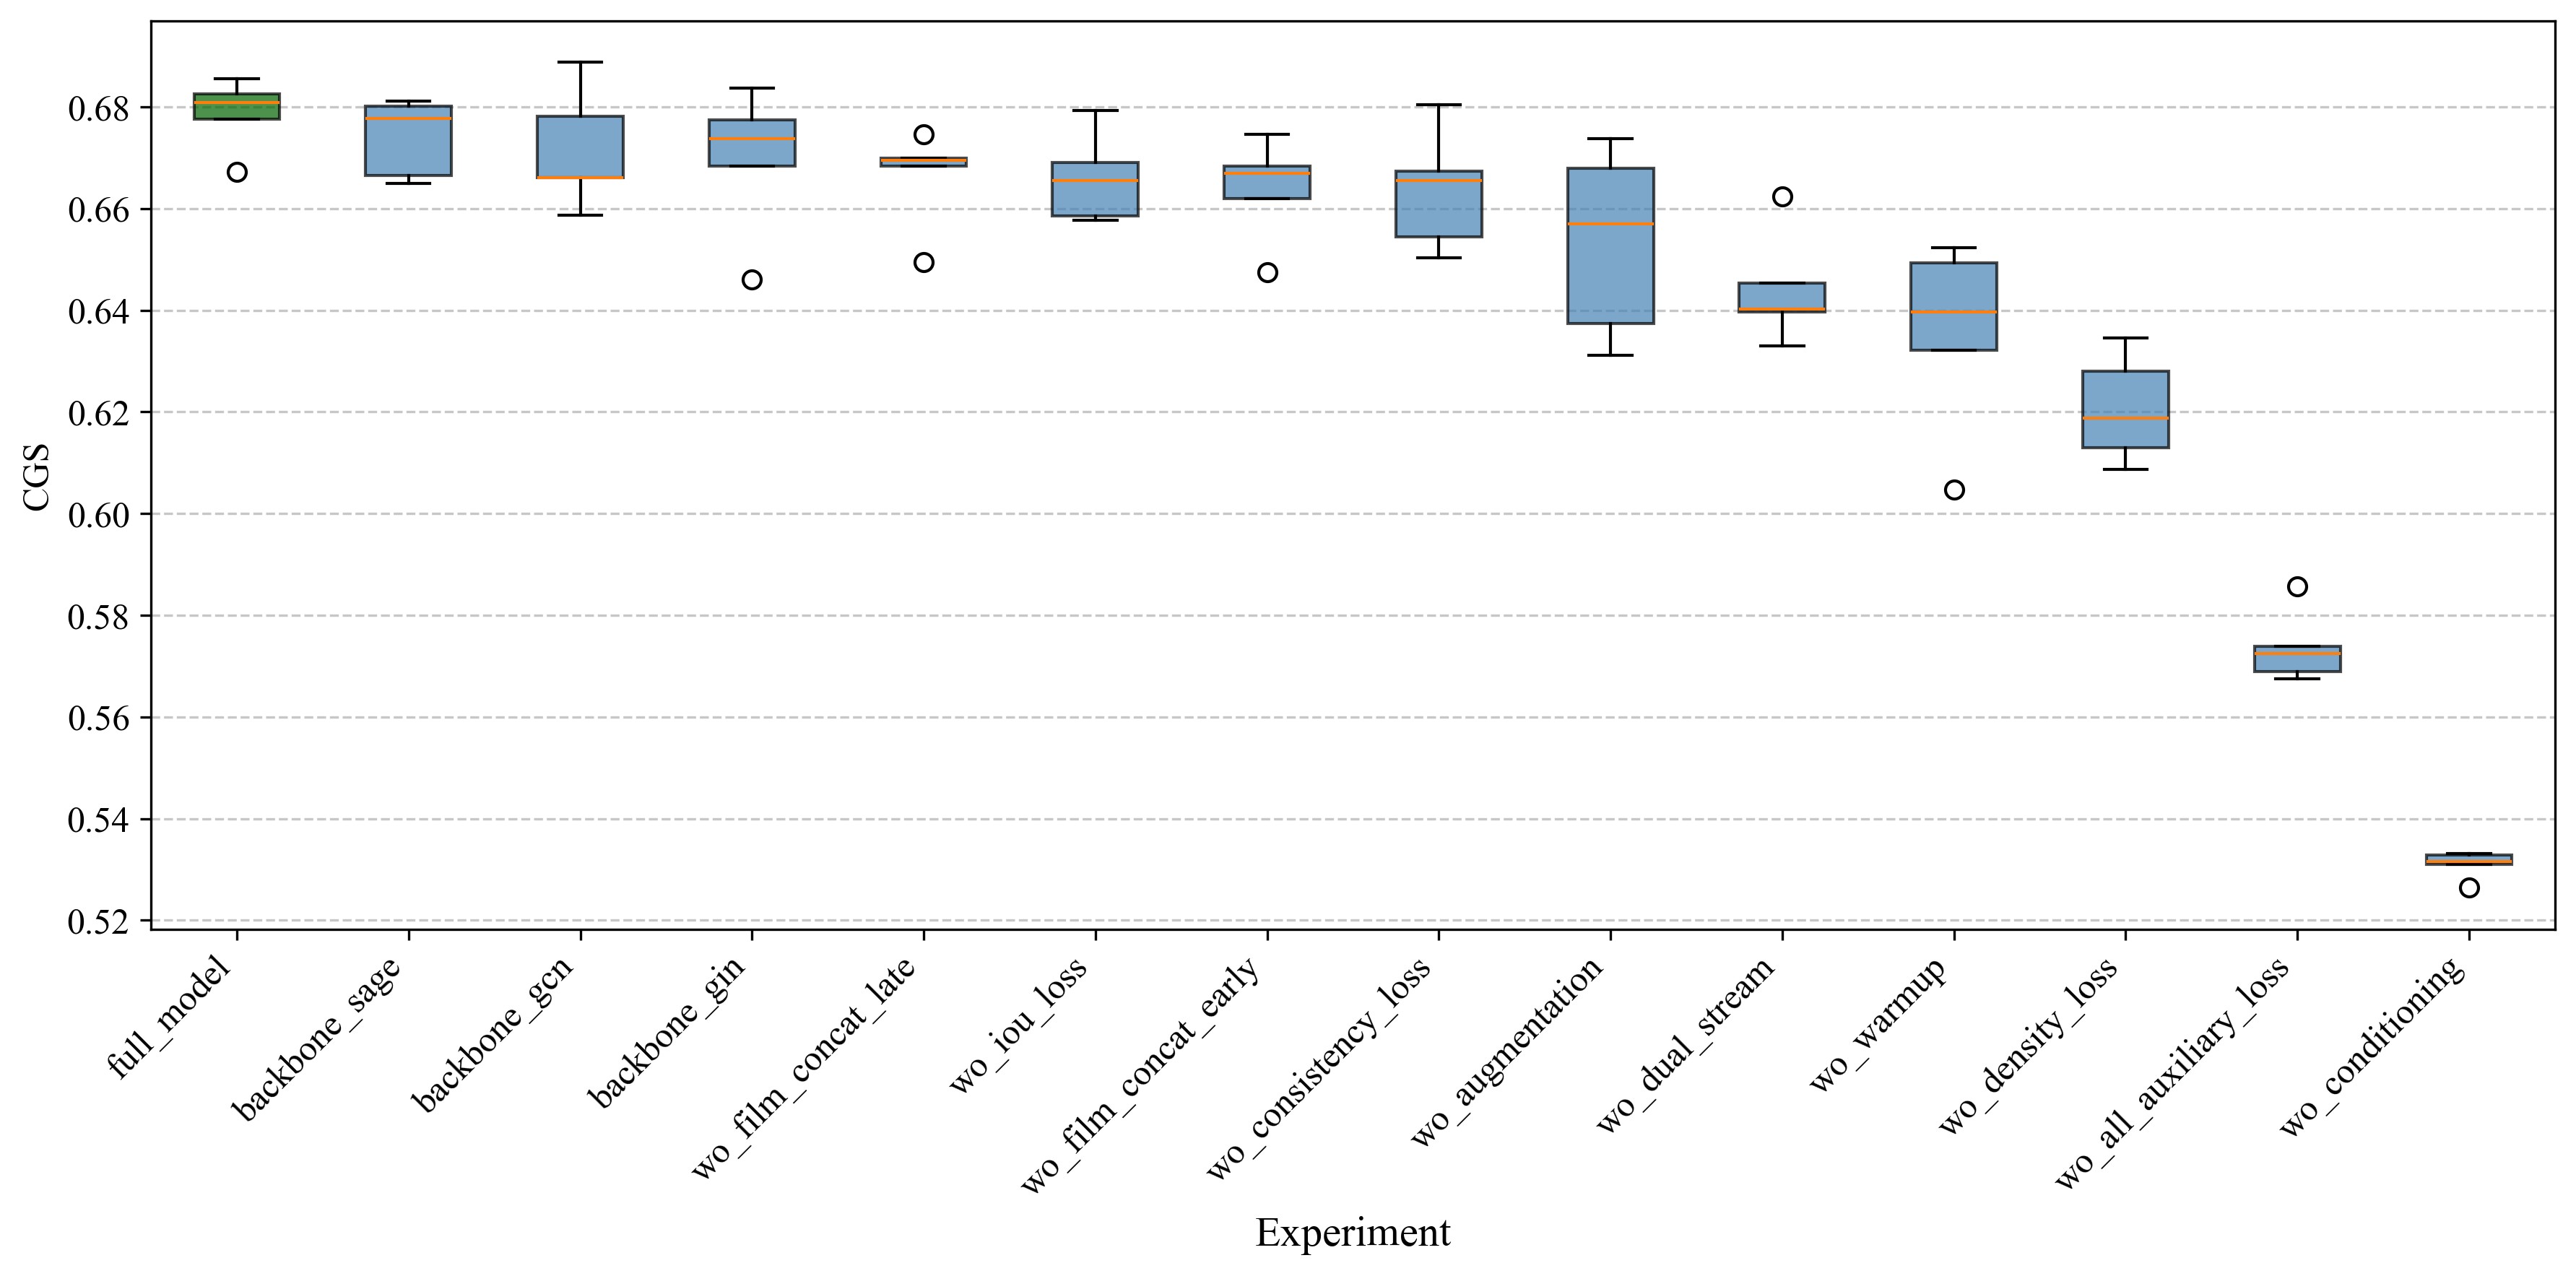
\includegraphics[width=0.92\textwidth]{boxplot.png}
\caption{Boxplot of CGS across 5-fold cross-validation for the full model and ablation variants, sorted by mean CGS.}
\label{fig:ablation_boxplot}
\end{figure*}



\begin{table*}[t]
\caption{Performance comparison between room-based GNN (ours) and component-based GNN (Baseline) across metrics}
\label{tab:main_results}

\centering
% 定义居中对齐、可自动换行的 X 列类型（用于数值列）
\newcolumntype{C}{>{\centering\arraybackslash}X}

\begin{tabularx}{\textwidth}{l*{7}{C}}   % 第一列左对齐，后面7列居中对齐并自动撑满
\toprule
\textbf{Method} & 
\textbf{Image IoU}$\uparrow$ & 
\textbf{Precision}$\uparrow$ & 
\textbf{Recall}$\uparrow$ & 
\textbf{F1}$\uparrow$ & 
\textbf{Accuracy}$\uparrow$ & 
\textbf{MAE}$\downarrow$ & 
\textbf{RMSE}$\downarrow$ \\
\midrule
\textcolor{red}{\textbf{Ours}}      & \textcolor{red}{\textbf{0.565 $\pm$ 0.005}} & \textcolor{red}{\textbf{0.749 $\pm$ 0.010}} & \textcolor{red}{\textbf{0.781 $\pm$ 0.009}} & \textcolor{red}{\textbf{0.765 $\pm$ 0.001}} & \textcolor{red}{\textbf{0.771 $\pm$ 0.004}} & \textcolor{red}{\textbf{0.224 $\pm$ 0.006}} & \textcolor{red}{\textbf{0.370 $\pm$ 0.006}} \\
\textcolor{red}{\textbf{Baseline}}  & \textcolor{red}{0.454 $\pm$ 0.021}          & \textcolor{red}{0.638 $\pm$ 0.029}          & \textcolor{red}{0.625 $\pm$ 0.034}          & \textcolor{red}{0.630 $\pm$ 0.012}          & \textcolor{red}{0.619 $\pm$ 0.020}          & \textcolor{red}{0.376 $\pm$ 0.019}          & \textcolor{red}{0.578 $\pm$ 0.015}          \\
\textcolor{red}{\textbf{Diff(\%)}}      & \textcolor{red}{+11.07}         & \textcolor{red}{+11.10}         & \textcolor{red}{+15.67}         & \textcolor{red}{+13.49}         & \textcolor{red}{+15.20}         & \textcolor{red}{$\downarrow$15.27} & \textcolor{red}{$\downarrow$20.83} \\
\bottomrule
\end{tabularx}

\par\smallskip
{\small\noindent\parbox{\textwidth}{\raggedright \textcolor{red}{Note: Values are reported as mean $\pm$ standard deviation over the five fold checkpoints. $\uparrow$ indicates higher is better for classification metrics (Image IoU, Precision, Recall, F1, Accuracy); $\downarrow$ indicates lower is better for regression metrics (MAE, RMSE).}}}

\end{table*}


\begin{table*}[t]
\centering
\begingroup\color{red}
\caption{Graph complexity and computational efficiency comparison between the component-level and room-level representations}
\label{tab:efficiency}
\begin{tabular*}{\textwidth}{@{\extracolsep{\fill}}lccccc@{}}
\toprule
Method & Avg. nodes & Avg. edges & Inference time / plan & Training time / epoch & GPU memory \\
\midrule
Component-level GNN & 244 $\pm$ 14 & 444 $\pm$ 32 & 0.12 s & 103 s & 981 MB \\
Room-level GNN & 26 $\pm$ 4 & 71 $\pm$ 17 & 0.06 s & 86 s & 589 MB \\
Reduction & 89.3\% & 84.0\% & 50.0\% & 16.5\% & 39.9\% \\
\bottomrule
\end{tabular*}
\par\smallskip
{\small\noindent\parbox{\textwidth}{\raggedright Note: Node and edge statistics are computed on 112 training floor plans. Reduction is computed relative to the component-level baseline.}}
\endgroup
\end{table*}



\begin{figure*}[t]
\centering
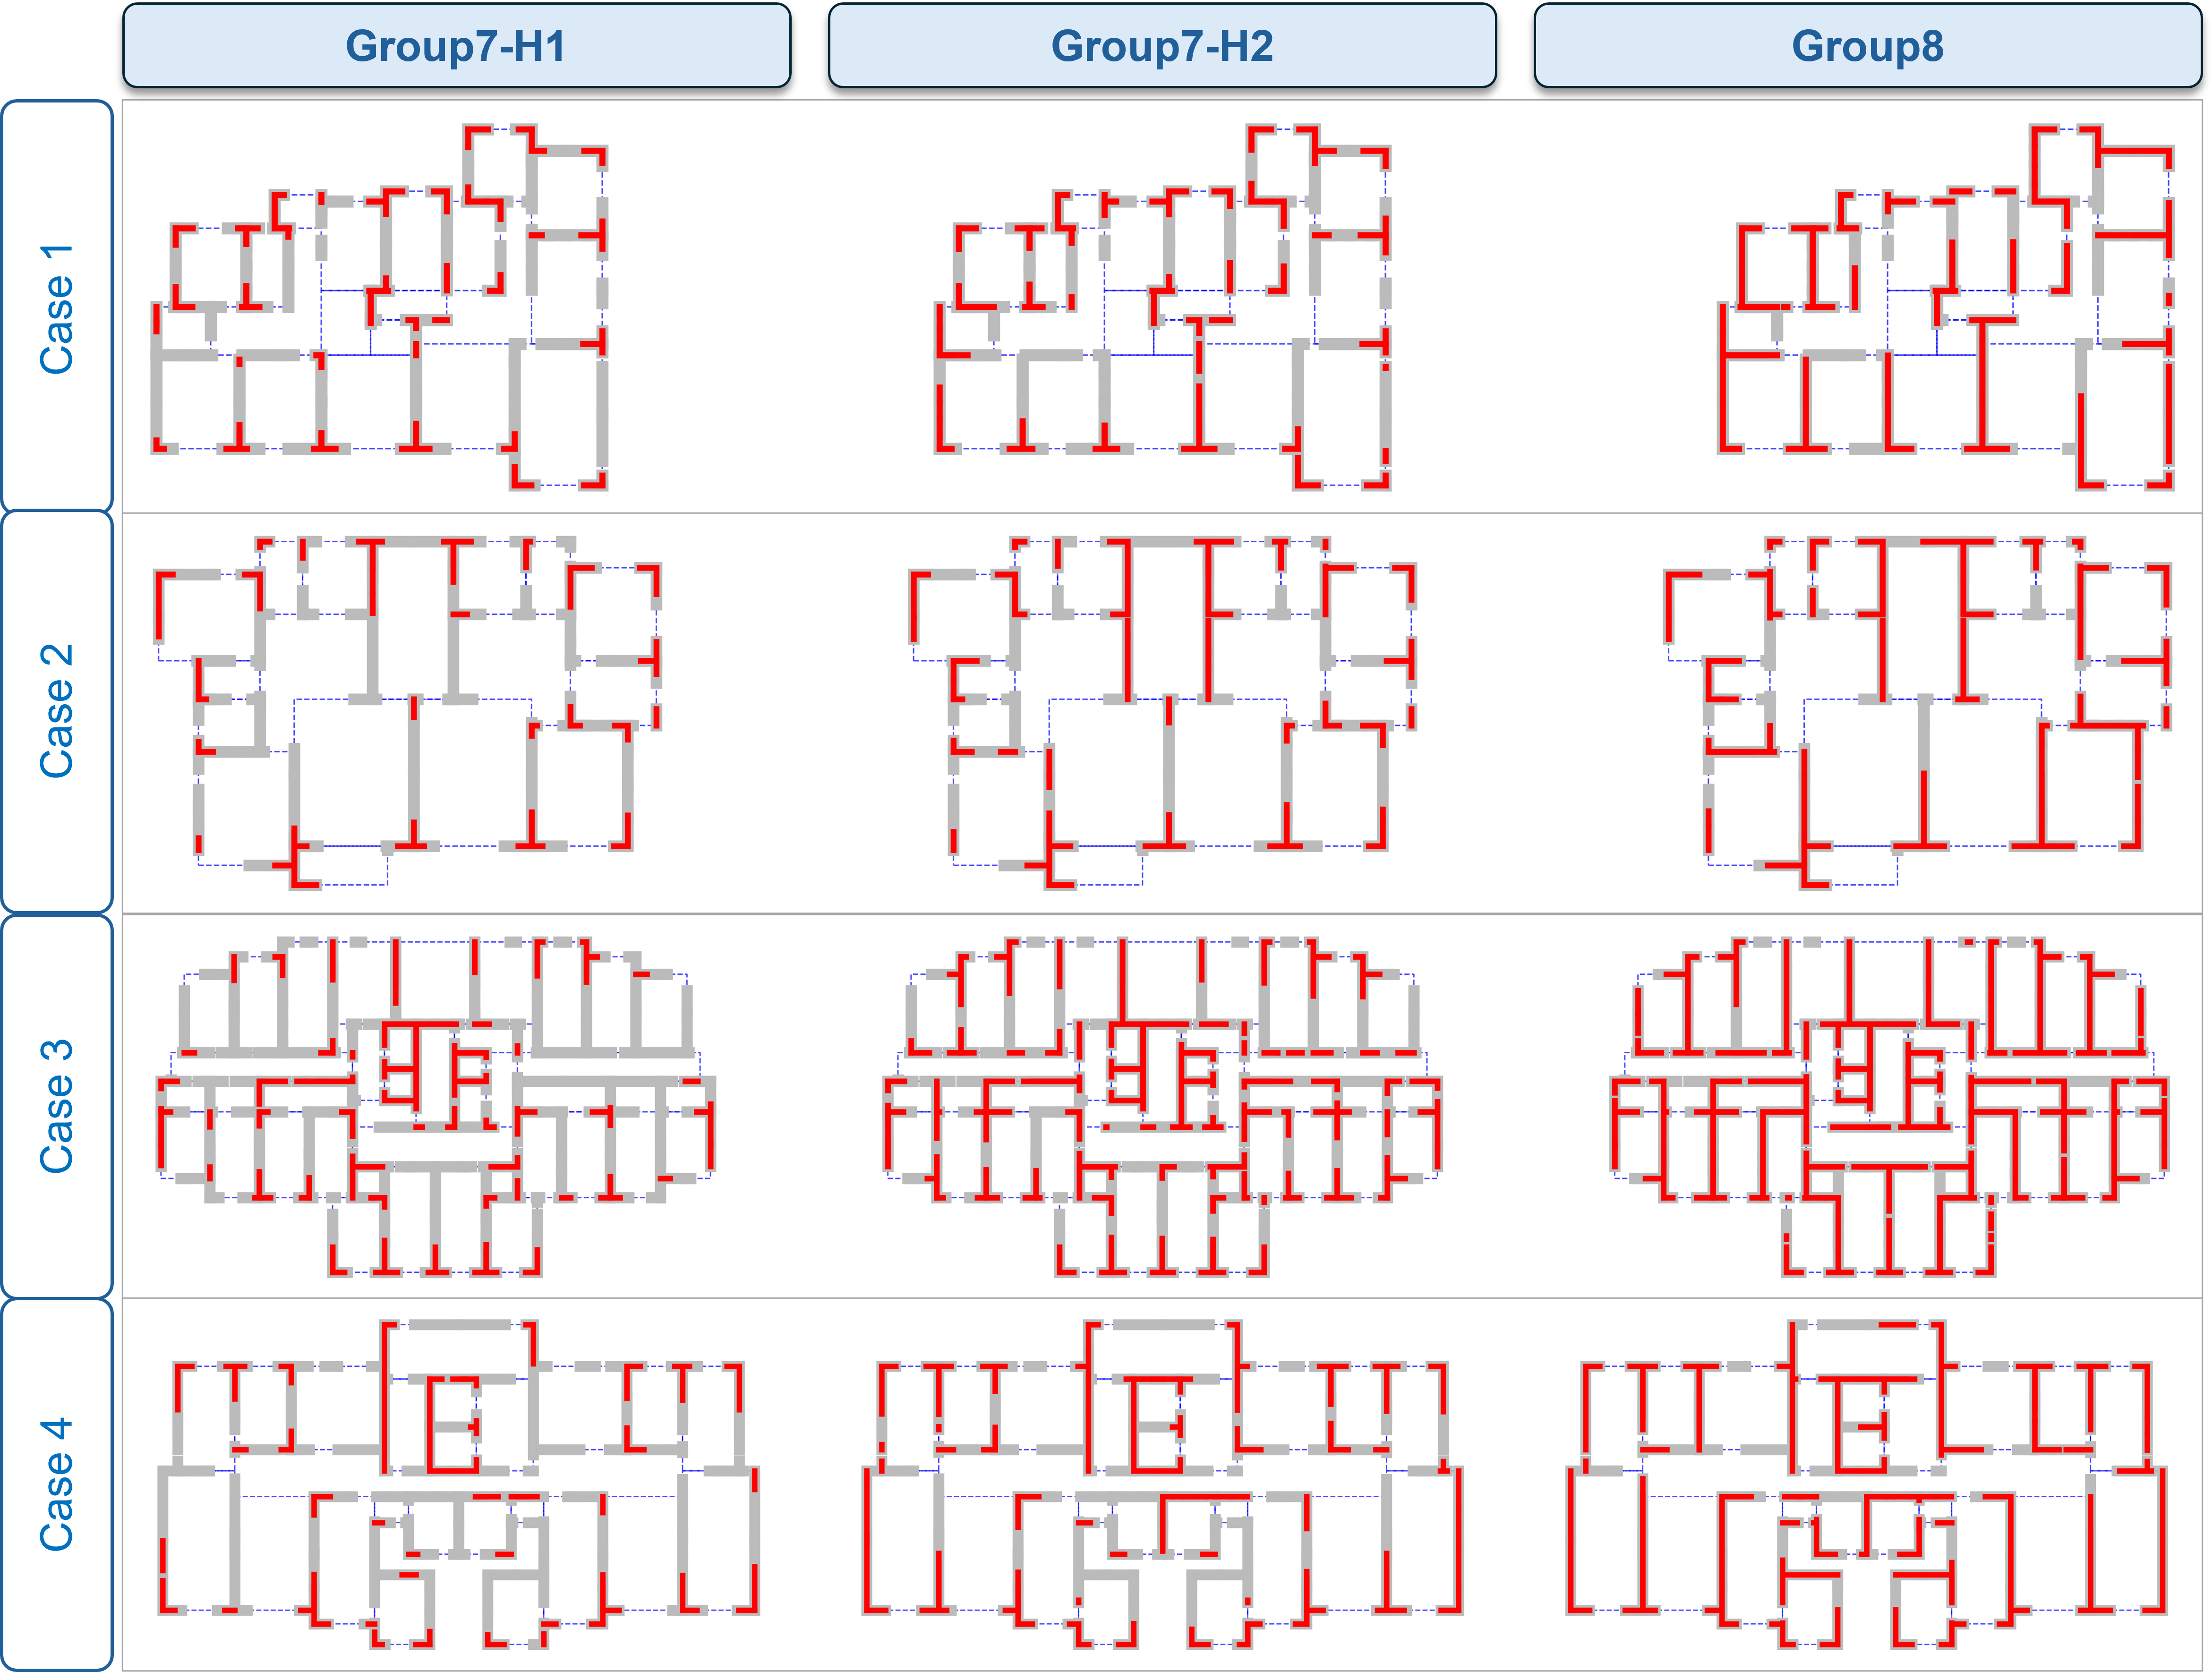
\includegraphics[width=0.9\textwidth]{conditional_gen.png}
\caption{Comparison of conditional generation results under different density conditions.}
\label{fig:conditional_gen}
\end{figure*}

\begin{figure*}[t]
\centering
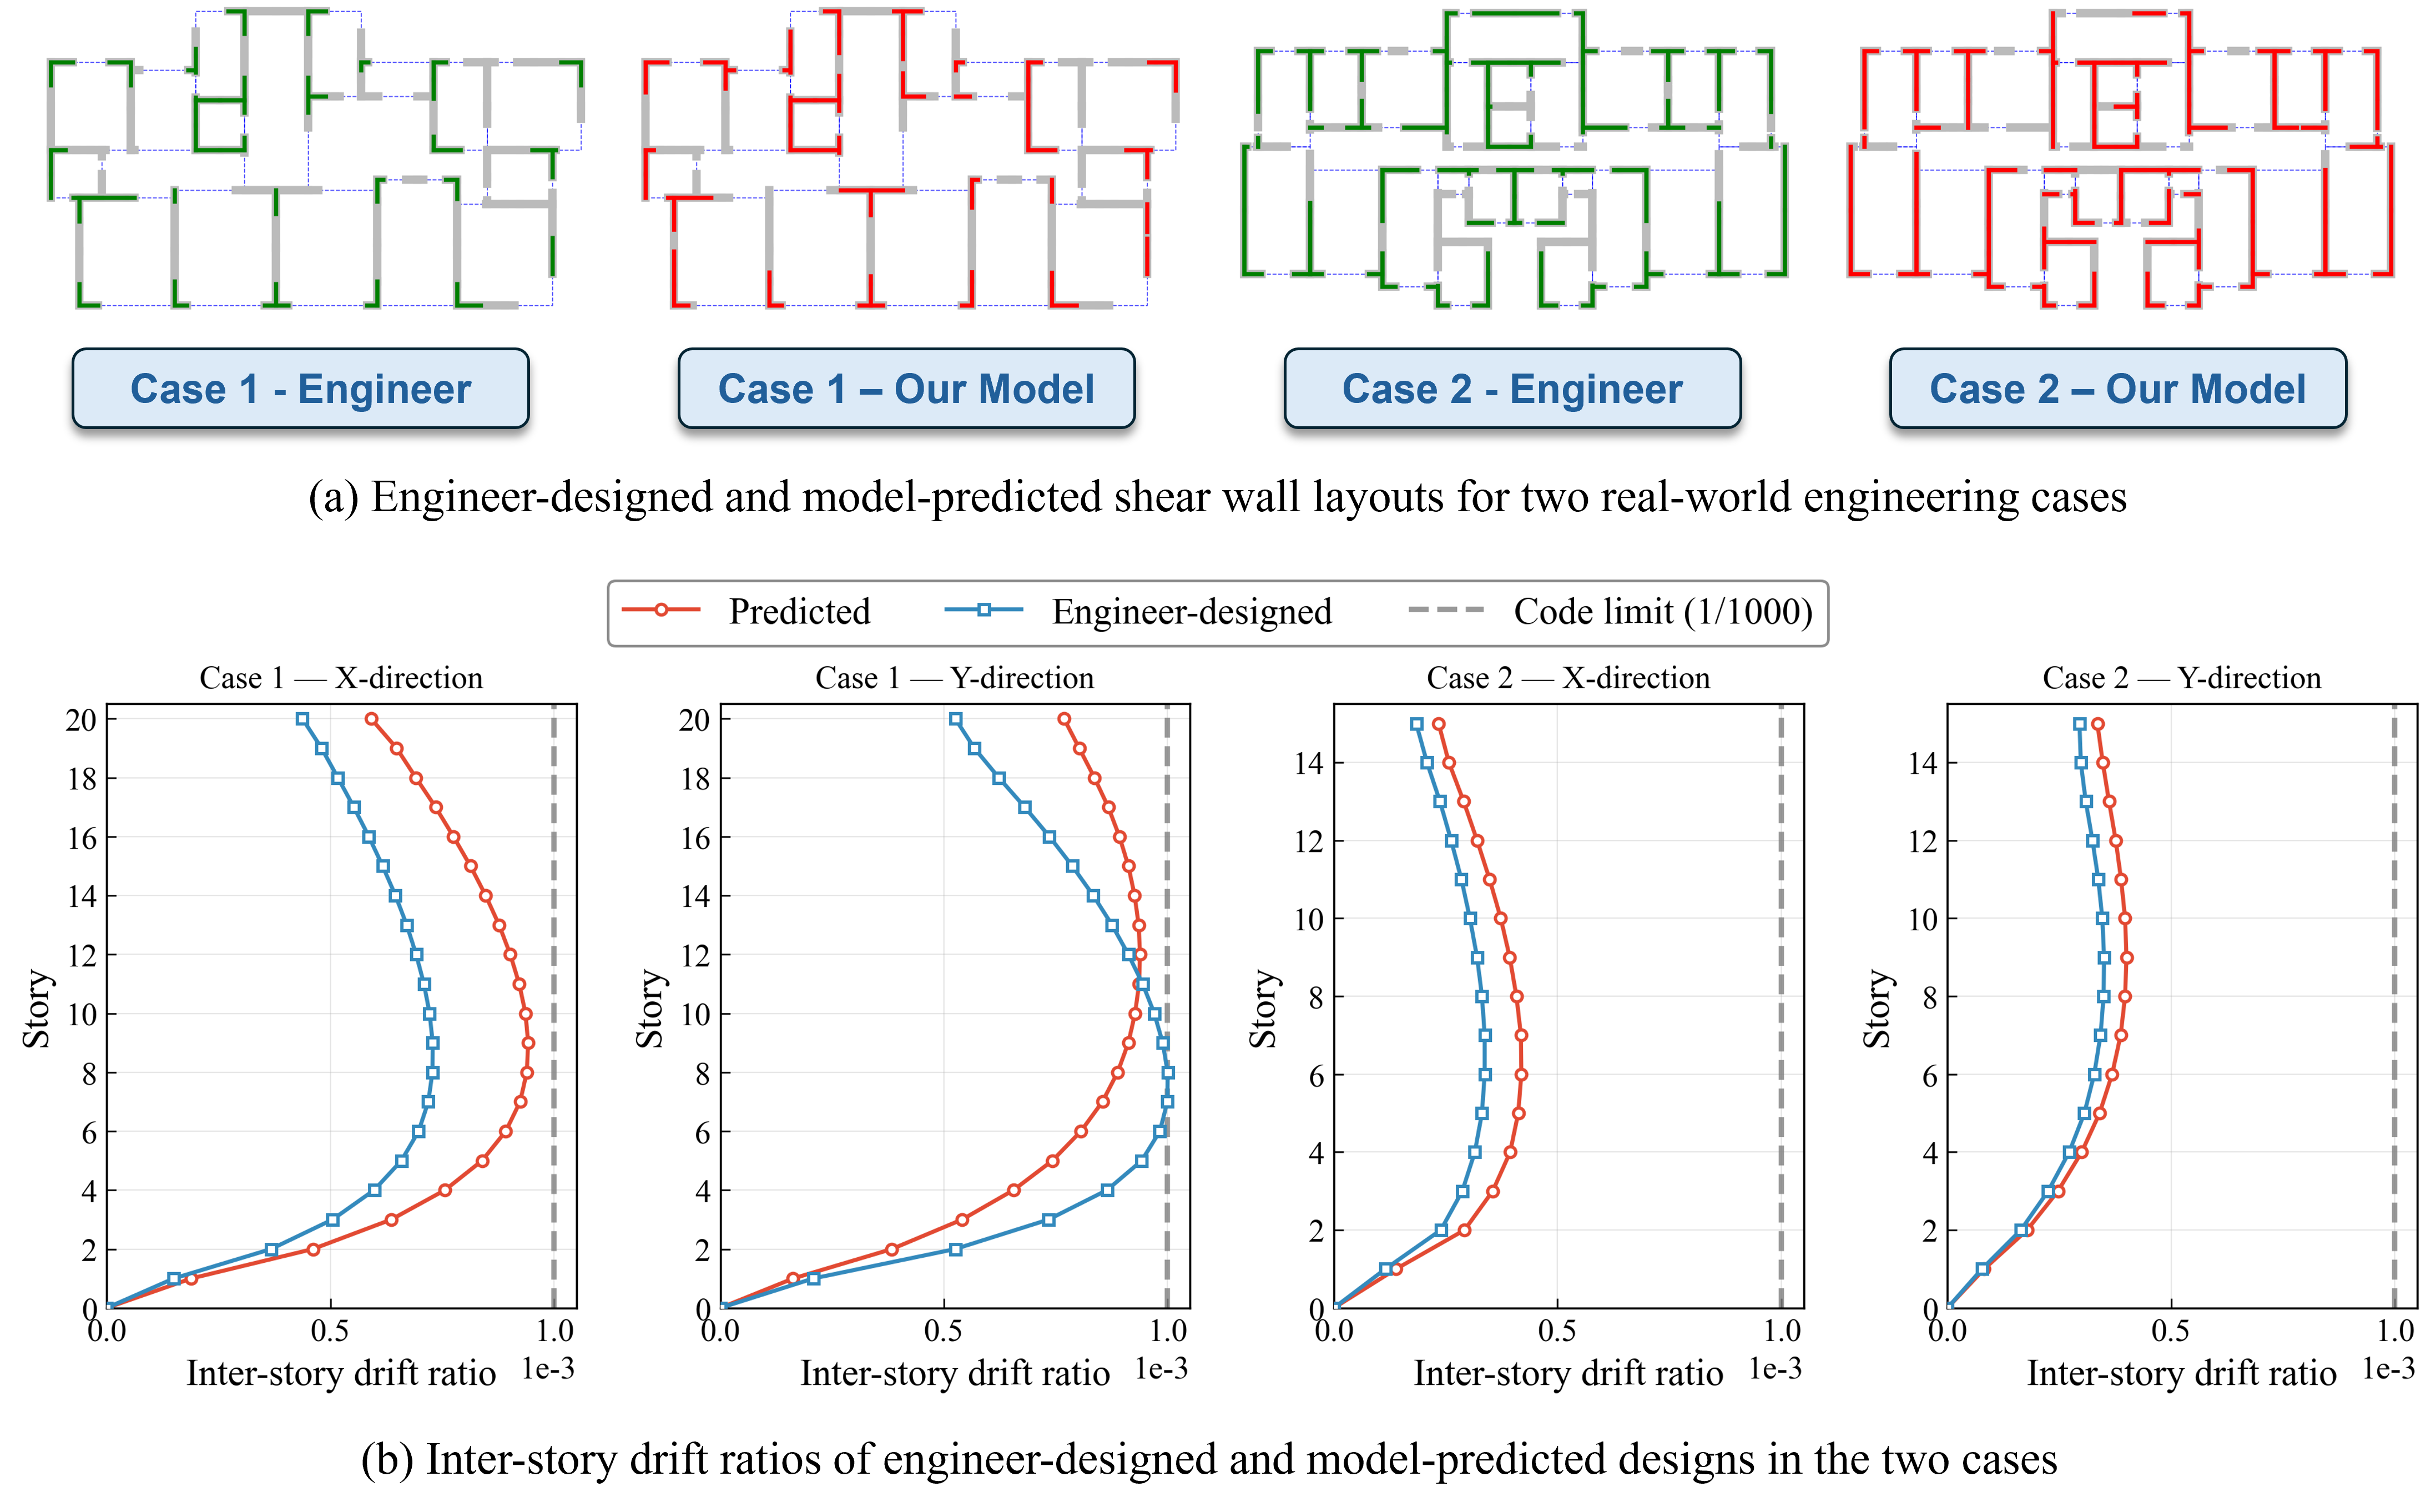
\includegraphics[width=\textwidth]{case_study.png}
\caption{Comparison of engineering validation results for two real projects.}
\label{fig:case_study}
\end{figure*}

\begin{figure*}[t]
\centering
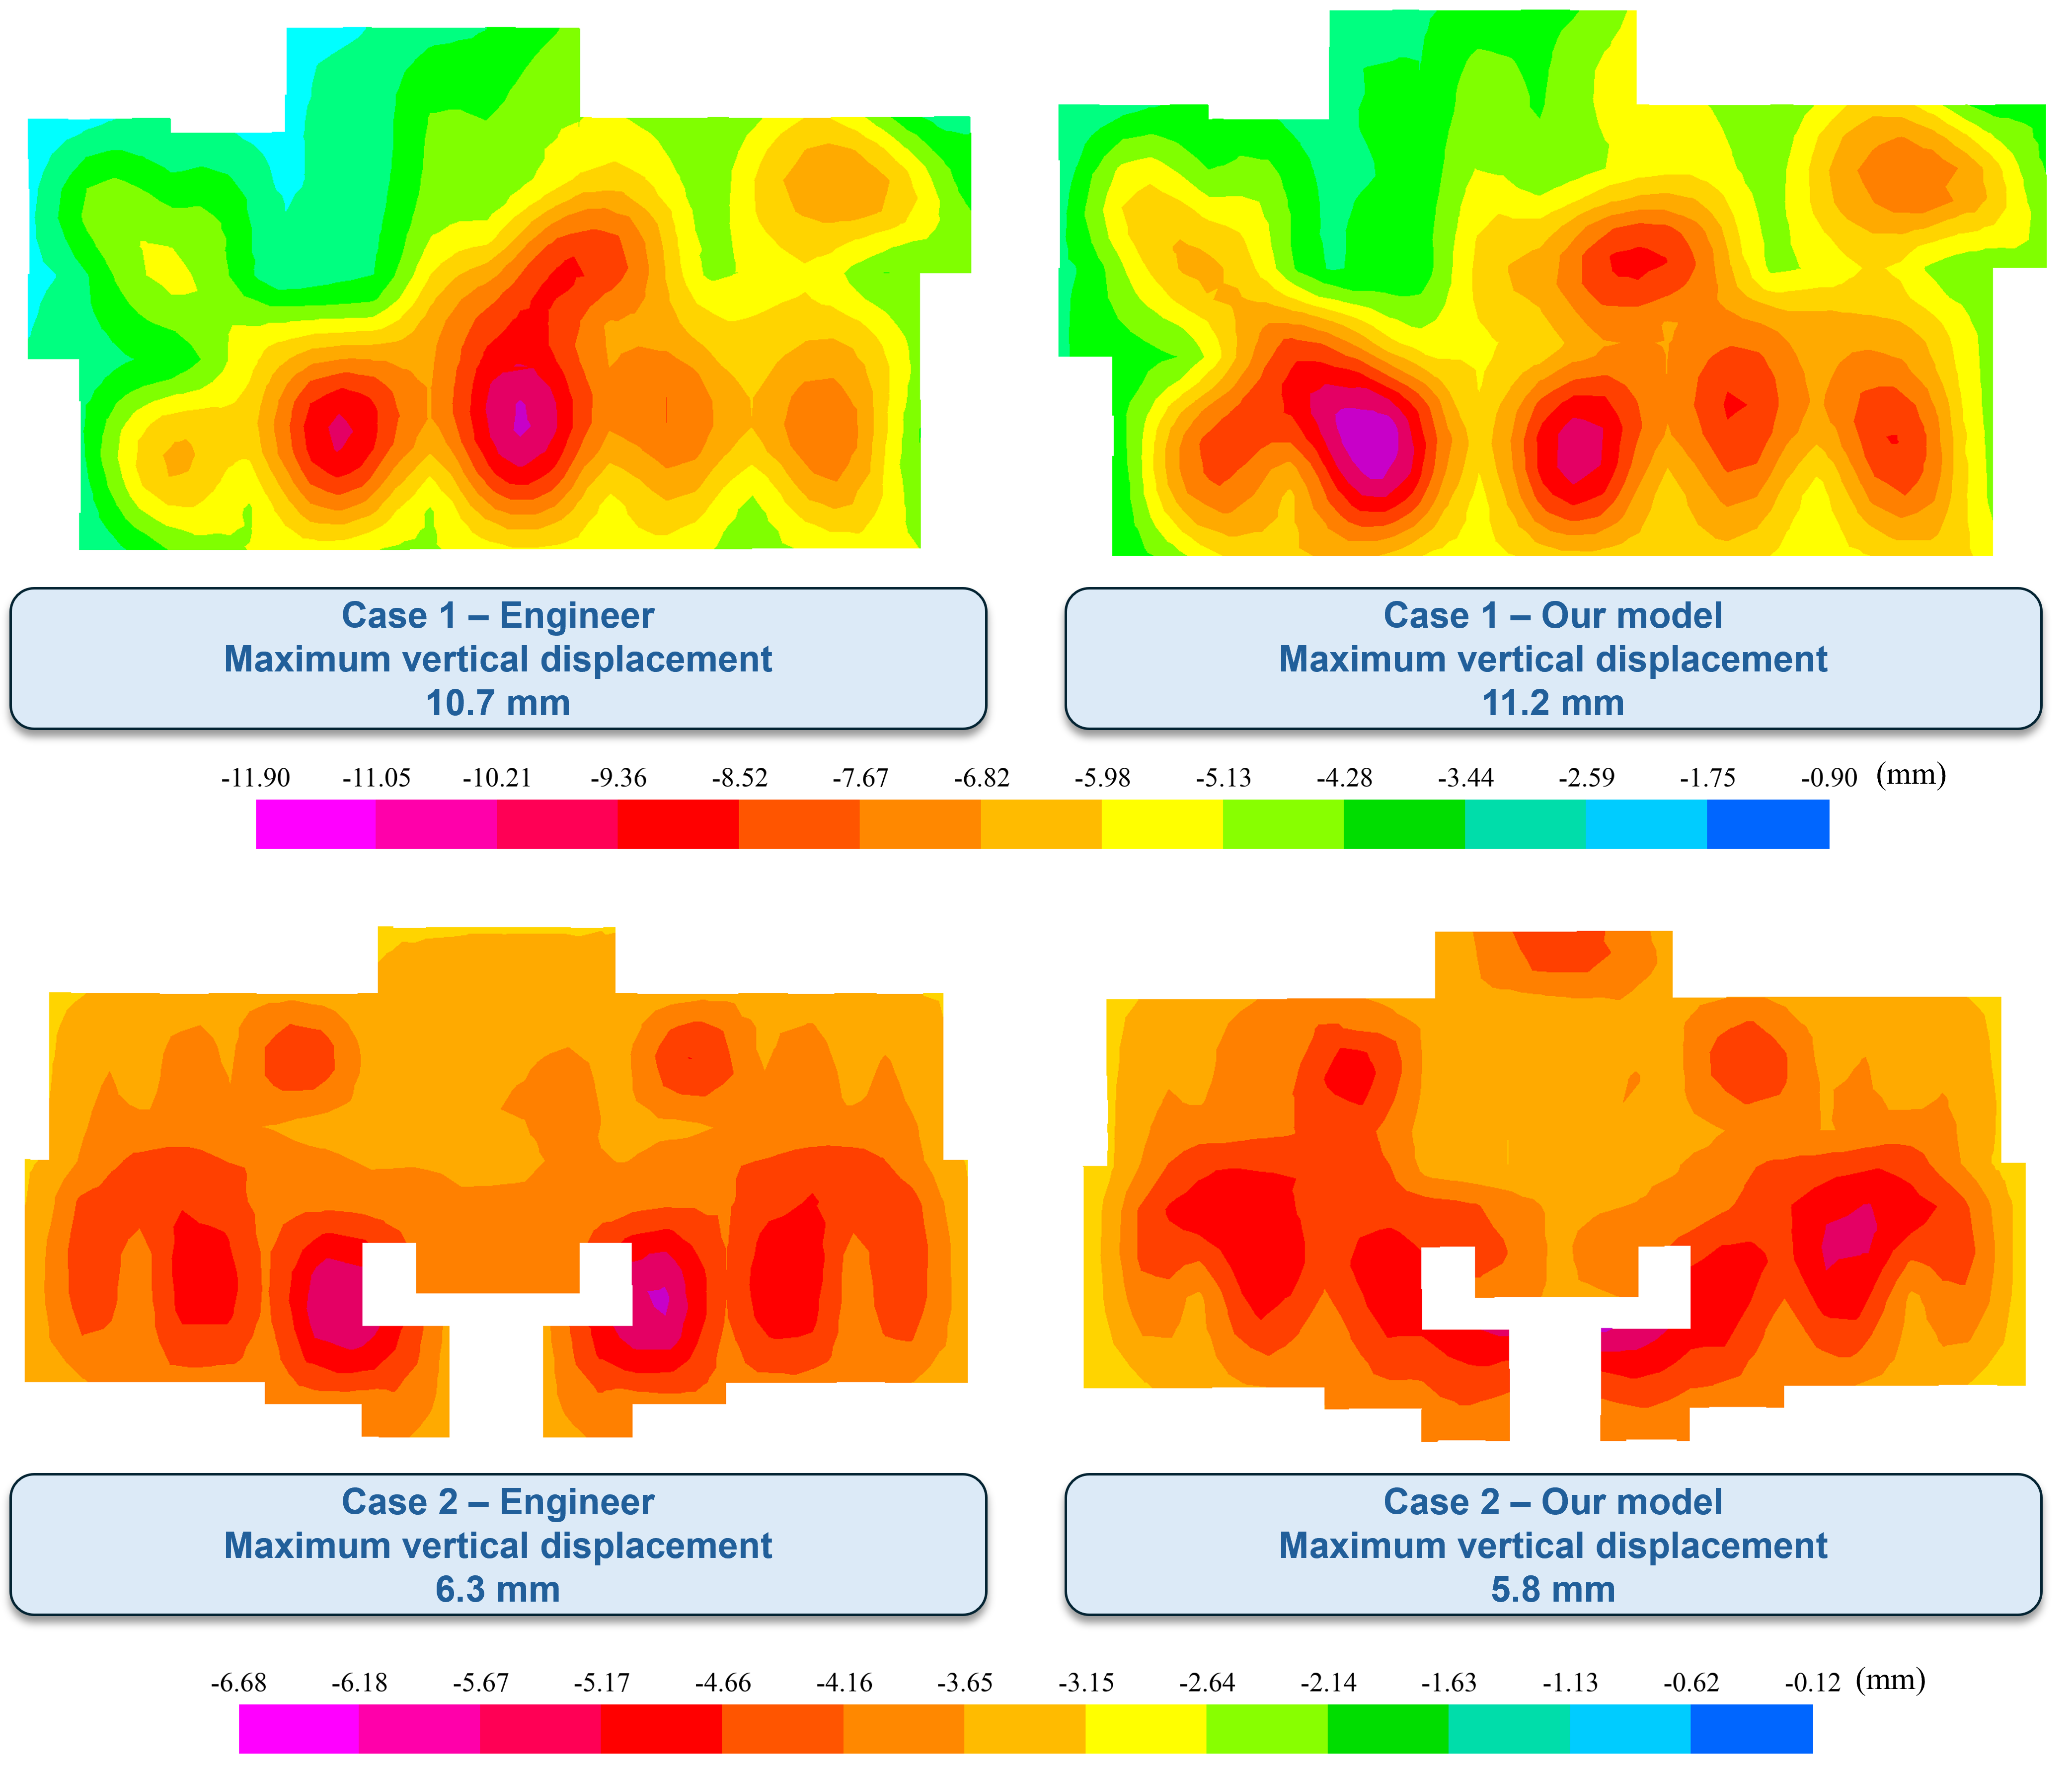
\includegraphics[width=0.85\textwidth]{vertical_disp_cloud_diagram.png}
\caption{Comparison of vertical displacement cloud diagrams for two real projects.}
\label{fig:vertical_disp_cloud}
\end{figure*}

A dataset of 143 high-rise residential floor plans is constructed from two sources: the open-source shear wall dataset reported by Liao et al. \cite{liaoAutomatedStructuralDesign2021a} and engineering drawings provided by Tongji Architectural Design (Group) Co., Ltd. In both sources, each retained sample contains an architectural floor plan and the corresponding shear wall layout designed by licensed structural engineers. The dataset used in this study is restricted to plans for which the architectural drawing, the engineered shear wall drawing, and the condition label can be aligned reliably after preprocessing; samples with incomplete drawings, ambiguous room partitioning, or invalid room-boundary extraction are excluded. Raw CAD drawings are processed through contour extraction and semantic partitioning to identify rooms and are then converted into the room-based graph representation described in Section~\ref{subsec:room_graph}. Because the public and proprietary data sources are subject to different sharing restrictions, we report the aggregated statistics of the combined dataset in Table~\ref{tab:dataset_stats}.

Following the condition taxonomy introduced in prior shear wall studies \cite{zhaoIntelligentDesignShear2023b}, which groups projects by the combined effects of seismic intensity and structural height, samples are categorized into three design-condition groups: the low-density group (Group7-H1), corresponding to seismic intensity 7 (PGA = 0.10\,g) and buildings with height $H \le 50$~m; the medium-density group (Group7-H2), sharing the same seismic intensity but covering buildings with $H > 50$~m; and the high-density group (Group8), corresponding to seismic intensity 8 (PGA = 0.20\,g). This grouping is used because the available dataset does not provide a sufficiently dense sampling of continuous design parameters for direct regression. \textcolor{red}{The three groups are defined before model training and are used as discrete condition inputs throughout the experiments.}

\textcolor{red}{It should be noted that the condition label used in this study is a discrete density category rather than a continuous engineering descriptor. Therefore, the model learns to respond to low-, medium-, and high-density regimes, but it does not directly condition on continuous parameters such as PGA, structural height, fundamental period, inter-story drift demand, or torsional response.}



\subsubsection{Baseline}
\label{subsubsec:baselines}

To assess the impact of the proposed room-based representation, performance is compared against a representative component-based GNN baseline consistent with prior studies \cite{zhaoIntelligentDesignShear2023b,zhaoDesignconditioninformedShearWall2023d}. For the baseline, graphs are constructed using wall intersection points as nodes and wall segments as edges, and the model regresses continuous wall-coverage ratios for each segment, where two values are predicted to describe coverage measured from the two endpoints of the wall segment.

To isolate the effect of representation, the modeling and training configuration is kept comparable across methods: both use the same backbone family (GATv2), follow the same training schedule, apply the same data augmentation strategy, and adopt the same cross-validation protocol, with hyperparameters tuned on their respective validation sets. For the baseline, conditioning is incorporated by concatenating the design-condition embedding to both node and edge feature vectors, following the feature-concatenation strategy adopted in prior component-based formulations. Because the open-source dataset does not provide continuous design parameters (e.g., PGA, site period, building height), the condition is represented as a one-hot encoded categorical variable corresponding to the three design groups, ensuring consistency with the available data.

\textcolor{red}{The experimental comparison focuses on graph-based methods because the central question of this study is whether a room-level graph representation can improve graph-based shear wall layout prediction compared with the commonly used component-level graph representation. Pixel-based GAN or diffusion models follow a substantially different formulation, where both inputs and outputs are raster images and predicted wall layouts require additional vectorization before engineering analysis. A direct comparison with such models would involve differences in representation, post-processing, resolution, and evaluation pipeline, making it difficult to isolate the effect of graph representation. Therefore, the component-level GNN is selected as the primary baseline to provide a controlled comparison at the representation level.}


\subsubsection{Implementation details and training settings}
\label{subsubsec:implementation}

The proposed room-based model uses a hidden dimension of 256 and a 32-dimensional condition embedding. The GNN encoder contains three GATv2 layers with four attention heads per layer and a dropout rate of 0.2. Models are trained with AdamW for 100 epochs using a cosine-annealing learning-rate schedule with a 20-epoch warmup; the batch size is one graph per iteration. The main optimization hyperparameters are selected by validation-set performance within each fold. In particular, the learning rate is chosen from $\{1\times10^{-4}, 5\times10^{-4}, 1\times10^{-3}\}$ and the weight decay from $\{0, 1\times10^{-5}, 1\times10^{-4}\}$; the final setting of learning rate $1\times10^{-3}$ and weight decay $1\times10^{-4}$ gives the most stable convergence and the best validation IoU in our pilot runs. At inference time, a classification threshold of 0.5 is used for wall existence prediction, and a ratio threshold of 0.1 is applied when converting regressed segment ratios into final layout elements.

To improve generalization under limited data, standard geometric augmentations are applied to each training sample, including horizontal/vertical flips and rotations by 90$^{\circ}$, 180$^{\circ}$, and 270$^{\circ}$, with output labels transformed accordingly. \textcolor{red}{To avoid data leakage, the dataset split was performed at the original floor-plan level before data augmentation. All augmented variants of the same original floor plan were kept within the same subset. In each subset, geometric augmentation was applied only to the training portion, while validation and test layouts were never included in the training set in either original or augmented form.} And to mitigate the imbalance among design conditions (Low:Medium:High = 33:52:58), weighted random sampling is adopted so that each epoch observes a more balanced mixture of conditions, following common practices for imbalanced deep learning problems.

For generalization and robust reporting, 5-fold cross-validation is employed. In each fold, 80\% of the data are used for model development and 20\% for testing; within the development split, 10\% of the training portion is held out for validation, and early stopping is applied with a patience of 20 epochs based on validation IoU \cite{Berrar_2019}. All experiments use a consistent preprocessing pipeline and the same split protocol across compared methods.

All experiments are conducted on a workstation equipped with an Intel Core i7-12700F CPU, 32\,GB RAM, and an NVIDIA RTX 3060 GPU (12\,GB). The implementation is based on Python 3.12, PyTorch 2.5.1.


\subsubsection{Evaluation metrics}

(1) Geometric accuracy. For evaluation consistency across representations, predictions from both methods are rasterized into binary layout images and compared using Image IoU, which measures pixel-level overlap between predicted and reference shear wall visualizations. Image IoU is used as the primary metric:
\begin{equation}
\text{Image IoU}=\frac{|P\cap G|}{|P\cup G|}
\end{equation}
where $P$ and $G$ denote the predicted and ground-truth positive pixel sets, respectively. This image-based evaluation enables a representation-agnostic comparison across methods.

For the room-based method, a vector-level IoU is additionally reported on the 16-dimensional output parameterization to quantify parametric overlap without rasterization. Segment-level precision/recall/F1 are computed by thresholding predicted/ground-truth segment values at 0.1, consistent with the inference rule used to convert ratios into final wall elements:
\begin{align*}
\text{Precision}&=\frac{TP}{TP+FP}, \quad
\text{Recall}=\frac{TP}{TP+FN}, \quad
\text{F1}=\frac{2PR}{P+R}.
\end{align*}
where $TP$, $FP$, and $FN$ denote true positives, false positives, and false negatives, respectively, and $P$ and $R$ denote precision and recall.
For correctly identified positive segments, MAE is used to evaluate the error of predicted length ratios \cite{Chai_2014}:
\begin{equation}
\text{MAE}=\frac{1}{|S^+|}\sum_{(i,j)\in S^+}|\hat y_{ij}-y_{ij}|.
\end{equation}
Here, $S^+$ denotes the set of buildable segments with positive ground-truth wall coverage.

(2) Conditional generation. Standard supervised metrics require matched ground-truth layouts and therefore cannot directly evaluate mismatched conditions (e.g., generating a high-density layout for a plan labeled as low-density). To characterize conditional behavior across all conditions, the Conditional Generation Score (CGS) is defined as
\begin{equation}
\text{CGS}=w_1 S_{\text{den}}+w_2 S_{\text{IoU}}+w_3 S_{\text{uni}}.
\end{equation}
Here, $S_{\text{den}}$ measures agreement with target density statistics:
\begin{equation}
S_{\text{den}}=1-\frac{|\bar\rho_{\text{pred}}-\bar\rho_{\text{target}}|}{\bar\rho_{\text{target}}}.
\end{equation}
$S_{\text{IoU}}$ corresponds to Image IoU when the generated condition matches the ground-truth label. $S_{\text{uni}}$ summarizes spatial rationality by combining global variation, local smoothness across adjacent rooms, and penalties for extreme outliers:
\begin{equation}
S_{\text{uni}}=\alpha_1(1-c_v)+\alpha_2 s+\alpha_3(1-o).
\end{equation}
Here, $c_v$ is the coefficient of variation, $s$ is the local smoothness score, and $o$ is the outlier ratio. \textcolor{red}{In the main ablation analysis, the CGS weights are set to $(w_1,w_2,w_3)=(0.4,0.4,0.2)$. This setting gives comparable emphasis to density compliance and matched-condition geometric agreement, while assigning a smaller but non-negligible weight to spatial uniformity. The rationale is that the first two terms directly measure whether the generated layout follows the specified design condition and matches the engineer-designed layout under the true condition, whereas $S_{\text{uni}}$ acts mainly as a regularity check that penalizes highly uneven or locally erratic distributions. CGS is therefore used as a descriptive composite score rather than as a code-prescribed engineering index. To check that the ablation conclusions are not overly dependent on this particular choice, Table~\ref{tab:cgs_sensitivity} reports CGS values under several alternative component weights. The relative trends remain largely stable: the full model stays among the strongest variants, and it consistently outperforms the variants without dual-stream training and without density loss.} The coefficients in $S_{\text{uni}}$ are set to $(\alpha_1,\alpha_2,\alpha_3)=(0.4,0.4,0.2)$ to place comparable emphasis on global variation and local smoothness, while assigning a smaller but non-negligible weight to the outlier penalty.


As a complementary metric, the $Score_{\text{DC}}$ indicator proposed by Zhao et al. \cite{zhaoDesignconditioninformedShearWall2023d} is additionally reported. Score$_{\text{DC}}$ evaluates both layout overlap similarity and shear wall ratio similarity by weighting IoU$_{\text{SW}}$ with directional density-consistency terms:
\begin{equation}
\text{Score}_{\text{DC}} = \text{IoU}_{\text{SW}} \cdot \left(1-\frac{|\rho_x^{\text{pred}}-\rho_x^{\text{gt}}|}{\rho_x^{\text{gt}}}\right) \cdot \left(1-\frac{|\rho_y^{\text{pred}}-\rho_y^{\text{gt}}|}{\rho_y^{\text{gt}}}\right)
\end{equation}
In this expression, $\rho_x$ and $\rho_y$ denote shear wall density ratios along two orthogonal directions. Therefore, Score$_{\text{DC}}$ decreases when either overlap quality or directional density consistency deteriorates.

It should be noted that $S_{\text{den}}$ relies on target densities $\bar\rho_{\text{target}}$ estimated for each design condition and therefore reflects dataset-specific distributions rather than absolute engineering requirements. \textcolor{red}{In our implementation, the target densities used in both the density loss and CGS evaluation are fixed group-level averages computed from the complete set of available layouts after condition grouping, rather than being recomputed separately within each cross-validation fold.} From a structural engineering perspective, higher seismic intensity and greater building height generally require increased lateral-load-resisting capacity, which typically manifests as higher shear wall ratios \cite{qianDesignTallBuilding2018}. The density term is therefore intended to assess whether generated layouts respond systematically to the specified condition, rather than to enforce a code-prescribed threshold. To reduce the risk that conclusions depend on a single composite metric, CGS together with its three sub-scores and the independent Score$_{\text{DC}}$ metric are reported.



\subsection{Main results}
\label{subsec:main_results}

Table~\ref{tab:main_results} reports the quantitative comparison between the proposed room-based GNN and the component-based GNN baseline.



\textcolor{red}{The proposed room-based representation yields higher fold-averaged Image IoU and F1 than the component-based baseline under the same backbone family and training protocol. Across the five fold checkpoints, the room-level model achieves an Image IoU of 0.565 $\pm$ 0.005 and an F1 score of 0.765 $\pm$ 0.001, compared with 0.454 $\pm$ 0.021 and 0.630 $\pm$ 0.012 for the component-level baseline. The smaller cross-fold variation of the proposed method suggests that the improvement is not dominated by a single favorable split. The ensemble result remains higher (Image IoU = 0.597), but Table~\ref{tab:main_results} reports fold-level statistics to make model stability explicit. The improvement is not only a numerical advantage but also a direct consequence of the representation level. In the component-based baseline, each wall segment is predicted largely as an individual unit, so locally plausible but globally inconsistent wall fragments can survive if nearby context is not aggregated effectively. In the room-based graph, by contrast, message passing occurs over room adjacencies and all candidate walls are attached to room boundaries from the outset. The model is therefore biased toward boundary-consistent predictions and is less likely to place isolated wall fragments in regions that do not correspond to valid room interfaces. This is important in engineering practice because fewer false positives mean lower unnecessary construction cost and fewer conflicts with architectural constraints. In addition, the lower MAE/RMSE indicates more accurate wall-length ratios for correctly identified segments, which is consistent with a representation that reasons over complete room boundaries rather than isolated wall segments.}

The qualitative comparisons in Fig.~\ref{fig:qual_comparison} provide visual evidence consistent with the quantitative results. \textcolor{red}{More illustrative examples can be seen in Fig.~\ref{fig:supp_case}.} Across different floor-plan cases, the room-based GNN generally produces wall layouts that are closer to the engineer-designed reference, with more coherent boundary-aligned wall placement and fewer spurious predictions. Correspondingly, the predicted layouts from the proposed method exhibit larger overlap with the ground truth, which is reflected in the higher Image IoU reported in Table~\ref{tab:main_results}. 

By contrast, the component-based baseline tends to generate more fragmented and isolated wall segments. These scattered predictions are especially visible in cases with complex room adjacencies, where local segment-level decisions do not fully capture the higher-level spatial organization of the floor plan. This qualitative failure mode is consistent with the lower representational level of the component-based graph. Because the model operates on individual wall components rather than room-level spatial units, it is more prone to producing locally plausible but globally incoherent wall fragments.


\begin{table*}[t]
\centering
\caption{Image IoU performance comparison by category}
\label{tab:per_condition}
\begin{tabular*}{\textwidth}{@{\extracolsep{\fill}} lrrrrr @{}}
\toprule
Category & \multicolumn{1}{c}{Ours Mean} & \multicolumn{1}{c}{Ours Std} & \multicolumn{1}{c}{Baseline Mean} & \multicolumn{1}{c}{Baseline Std} & \multicolumn{1}{r}{Improvement} \\
\midrule
Group7-H1 (Low)      & 0.5103 & 0.1120 & 0.3804 & 0.1001 & +34.14\% \\
Group7-H2 (Medium)   & 0.5975 & 0.0511 & 0.5168 & 0.0548 & +15.62\% \\
Group8 (High)   & 0.6473 & 0.0812 & 0.5523 & 0.0516 & +17.20\% \\
\midrule
Overall Average & 0.5850 & 0.0814 & 0.4832 & 0.0688 & +21.08\% \\
\bottomrule
\end{tabular*}
\end{table*}


\textcolor{red}{Table~\ref{tab:efficiency} provides a quantitative comparison of graph complexity and computational efficiency. The room-level representation reduces the average number of nodes from 244 to 26 and the average number of edges from 444 to 71, corresponding to reductions of 89.3\% and 84.0\%, respectively. This compact representation also improves efficiency in the measured implementation: inference time per plan decreases from 0.12~s to 0.06~s, training time per epoch decreases from 103~s to 86~s, and GPU memory usage decreases from 981~MB to 589~MB. These results support the claim that representing rooms rather than low-level wall components reduces graph complexity while lowering the computational cost of training and inference.}

\subsubsection{Per-condition results}

To examine whether performance is consistent across design conditions, Table~\ref{tab:per_condition} reports Image IoU stratified by condition.

The proposed method outperforms the component-based baseline in all three condition groups, indicating that the advantage of the room-level representation is not limited to a single density regime. The largest relative improvement is observed in the low-density group (Group7-H1, +34.14\%), where sparse wall distributions make false-positive predictions more detrimental to IoU. This pattern is mechanically consistent with the representation advantage discussed above. When the true layout contains relatively few walls, even a small number of spurious predicted segments occupies a large fraction of the union area and can sharply reduce IoU. The room-level formulation suppresses these false positives more effectively because it limits prediction to boundary-feasible locations and aggregates context at the room level, so the benefit becomes most visible in sparse-wall cases.

In absolute terms, the highest Image IoU is obtained in the high-density group (Group8, 0.6473), followed by the medium-density group (0.5975). Two factors likely contribute to this trend. First, the training data are imbalanced across categories (33:52:58), so the high-density category provides the largest number of examples from which the model can learn stable category-specific patterns. Second, denser layouts provide more continuous boundary-aligned wall patterns, which give both models stronger geometric supervision than sparse layouts. Even under these more favorable settings, however, the proposed method still maintains gains over the baseline, with improvements of 17.20\% and 15.62\% in the high- and medium-density groups, respectively. The role of data imbalance should therefore be interpreted as a contributing factor rather than a complete explanation.

The standard deviations also provide useful insight into robustness. Performance in the medium- and high-density groups is relatively stable across folds, whereas the low-density group shows larger variance for both methods. This suggests that sparse-layout cases are inherently more sensitive to sample composition and prediction thresholding, and that the smaller sample size of the low-density group further increases uncertainty. Nevertheless, the proposed method consistently preserves a margin over the baseline in every condition group, supporting the claim that the room-based formulation improves both average accuracy and cross-condition robustness.


\subsection{Ablation studies}
\label{subsec:ablation}

\newcolumntype{Y}{>{\centering\arraybackslash}X}

\begin{table*}[t]
\centering
\caption{Ablation study results}
\small
\label{tab:ablation}
\begin{tabularx}{\textwidth}{l *{5}{Y}}
\toprule
Configuration & CGS  & Density ($S_{den}$)  & IoU ($S_{IoU}$)  & Uniformity ($S_{uni}$)  & Score$_{\text{DC}}$ \\
\midrule
Full Model & 0.679 & 0.750 & 0.541 & 0.812 & 0.413 \\
\midrule
\textit{Conditioning Mechanism} & & & & & \\
w/o conditioning & 0.531 (-0.148) & 0.384 & 0.535 & 0.816 & 0.388 \\
w/o FiLM (concat early) & 0.664 (-0.015) & 0.745 & 0.482 & 0.865 & 0.349 \\
w/o FiLM (concat late) & 0.666 (-0.012) & 0.753 & 0.480 & 0.866 & 0.334 \\
\midrule
\textit{Loss Functions} & & & & & \\
w/o density loss & 0.621 (-0.058) & 0.607 & 0.542 & 0.805 & 0.427 \\
w/o IoU loss & 0.666 (-0.013) & 0.730 & 0.523 & 0.825 & 0.2763 \\
w/o consistency loss & 0.664 (-0.015) & 0.727 & 0.513 & 0.838 & 0.359 \\
w/o all auxiliary losses & 0.574 (-0.105) & 0.615 & 0.340 & 0.958 & 0.355 \\
\midrule
\textit{Training Strategy} & & & & & \\
w/o dual-stream & 0.644 (-0.035) & 0.772 & 0.366 & 0.945 & 0.394 \\
w/o warmup & 0.636 (-0.043) & 0.700 & 0.462 & 0.853 & 0.299 \\
w/o augmentation & 0.653 (-0.025) & 0.742 & 0.462 & 0.859 & 0.277 \\
\midrule
\textit{GNN Backbone} & & & & & \\
GCN & 0.672 (-0.007) & 0.751 & 0.507 & 0.842 & 0.292 \\
GraphSAGE & 0.674 (-0.005) & 0.749 & 0.519 & 0.835 & 0.349 \\
GIN & 0.670 (-0.009) & 0.756 & 0.496 & 0.845 & 0.312 \\
\bottomrule
\end{tabularx}
\end{table*}

Ablation experiments were conducted to quantify the contribution of each component. Table~\ref{tab:ablation} summarizes results using the Conditional Generation Score (CGS), its sub-metrics, and Score$_{\text{DC}}$.

Fig.~\ref{fig:ablation_boxplot} provides a complementary view of the same ablation results by visualizing the fold-wise CGS distribution of each variant. The most pronounced degradation occurs when conditioning is removed, where the CGS distribution shifts downward relative to the full model. This confirms that the conditioning mechanism is the primary basis for controllable generation rather than a marginal refinement.

The conditioning module accounts for the largest change in controllability-related performance. Removing conditioning reduces CGS by 0.148, driven primarily by a sharp drop in density consistency ($S_{den}$: 0.750 $\rightarrow$ 0.384), which indicates that outputs become less responsive to the specified design condition. This result follows the learning setup of the task. Geometry already explains much of the wall-layout pattern for a given floor plan, so when the condition input is removed, the network can still produce plausible layouts but loses a mechanism for systematically shifting wall quantity across density regimes. Among alternative injection strategies, FiLM yields small but consistent gains over early and late feature concatenation. This comparison is important because the baseline concatenation variants isolate the benefit of modulation-based condition injection from the effect of using condition inputs at all. The gain of FiLM suggests that repeatedly modulating intermediate features helps preserve the condition signal during deep propagation, whereas one-shot concatenation allows geometric features to dominate more easily.

\textcolor{red}{The loss-function ablations in Table~\ref{tab:ablation} and Fig.~\ref{fig:ablation_boxplot} demonstrate the roles of the density and consistency losses. Removing the density loss reduces CGS from 0.679 to 0.621, mainly because $S_{den}$ decreases from 0.750 to 0.607, indicating weaker compliance with the specified density condition. Removing the consistency loss reduces CGS from 0.679 to 0.664 and lowers the matched-condition IoU from 0.541 to 0.513, suggesting reduced coherence on shared room boundaries. Removing the IoU loss leads to a smaller CGS decrease (0.679 $\rightarrow$ 0.666), with $S_{IoU}$ decreasing from 0.541 to 0.523 and $S_{uni}$ increasing slightly from 0.812 to 0.825. However, its Score$_{\text{DC}}$ drops more noticeably from 0.413 to 0.276, indicating that the IoU term remains important for overlap-oriented layout quality even when the composite CGS changes modestly. The larger degradation observed when all auxiliary losses are removed further confirms that these losses provide complementary supervision for condition compliance and boundary consistency. The fact that the ranking trends remain consistent across CGS, its sub-scores, and Score$_{\text{DC}}$ supports the use of CGS as a summary indicator for conditional behavior in this study.}

Training-related components have moderate but non-negligible impacts. Eliminating the dual-stream strategy decreases CGS by 0.035, with the main change in $S_{IoU}$, consistent with improved condition sensitivity. Warmup contributes to optimization stability (CGS -0.043 without warmup). Data augmentation primarily benefits IoU (0.541 $\rightarrow$ 0.462 without augmentation). From the boxplot, both the "w/o augmentation" and "w/o warmup" variants exhibit visibly larger spread and more unstable fold-wise behavior than the full model, indicating that these components mainly improve robustness and consistency rather than only the best-case score.

For the GNN backbone, GATv2 achieves the best overall CGS; replacing it with GCN, GraphSAGE, or GIN results in consistent but modest decreases (approximately 0.005 to 0.009 in CGS). The small gaps among these backbones, together with the limited differences between early and late concatenation variants, suggest that the overall performance is driven more strongly by the representation, conditioning objective, and loss design than by a single specific graph convolution operator.

Finally, the full model not only attains the highest median CGS but also shows a comparatively compact distribution across folds. This indicates that the proposed combination of room-level representation, conditioning, and auxiliary objectives improves both average performance and training stability.



\subsection{Conditional generation analysis}
\label{subsec:conditional_analysis}

The ability to generate condition-dependent layouts is evaluated by applying all three condition inputs to the same set of floor plans.

\begin{table*}[t]
\centering
\caption{Density statistics by condition}
\label{tab:density_stats}
\begin{tabularx}{\textwidth}{XXXX}
\toprule
Input Condition & Target Density & Generated Density \newline (Mean $\pm$ Std) & Density Error(\%) \\
\midrule
Low (0) & 3.62 $\pm$ 1.02 & 3.42 $\pm$ 0.69 & 5.6 \\
Medium (1) & 4.89 $\pm$ 0.82 & 5.14 $\pm$ 1.01 & 5.0 \\
High (2) & 8.71 $\pm$ 1.04 & 7.96 $\pm$ 0.93 & 8.6 \\
\bottomrule
\end{tabularx}
\end{table*}

Fig.~\ref{fig:conditional_gen} shows that predicted layouts vary systematically across conditions, with denser wall coverage under more demanding settings. This trend is quantified in Table~\ref{tab:density_stats}, where the generated densities follow the intended order from low to high condition and remain within 8.6\% of the target values. Together, the visual and numerical results indicate that the model does not merely change local wall fragments, but adjusts the global amount of wall placement in a manner consistent with the prescribed condition.

\subsection{Case study: engineering validation}
\label{subsec:case_study}

To further verify engineering feasibility, two real projects outside the training set are selected for finite-element validation: Case 1 (story height 3.3\,m, 20 stories, seismic intensity 7) and Case 2 (story height 3.0\,m, 15 stories, seismic intensity 8). For each project, two structural schemes are analyzed under the same modeling assumptions: (i) the layout predicted by the proposed model and (ii) the reference layout designed by licensed engineers.

For both cases, room-based predictions are first converted into vector structural members and then imported into structural analysis software to build finite-element (FE) models. \textcolor{red}{The generated layout corresponds to one standard floor plan, and the same shear wall layout is assigned to all stories in each FE model. Therefore, vertical continuity is maintained in the analyzed cases, and no upper-story wall is suspended without a corresponding wall below.} Response-spectrum analysis is conducted to obtain inter-story drift ratios and displacement responses, consistent with standard seismic evaluation practice for building structures \cite{GB500112010Code2016,qianDesignTallBuilding2018}. \textcolor{red}{The comparison focuses on key preliminary-design indicators shown in Figs.~\ref{fig:case_study} and~\ref{fig:vertical_disp_cloud}, including the predicted and engineer-designed layouts, inter-story drift ratios, the code limit, and maximum vertical displacement.}

As shown in Fig.~\ref{fig:case_study}, the predicted schemes in both cases exhibit drift-ratio profiles close to those of the engineer-designed schemes, and all story drift ratios remain below the code limit of $1/1000$ \cite{GB500112010Code2016}. This result indicates that, for these two projects, the generated layouts maintain lateral stiffness at a level comparable to the reference schemes. Fig.~\ref{fig:vertical_disp_cloud} provides a consistent picture: the displacement cloud patterns of the predicted and engineer-designed schemes are similar, and the differences in maximum floor vertical displacement remain small. Taken together, these FE comparisons provide preliminary case-based evidence that the proposed method can generate structurally plausible layouts for high-rise residential projects of the tested types. They do not by themselves establish general validity across all building typologies, design codes, or seismic scenarios.
